%================================================================
% Detailed Solution Report Template
% Ice Ih Basal Surface: Proton Order via Monte Carlo Simulation
% 
% Fill in your own content where [TODO] appears.
% Compile with: pdflatex -> bibtex -> pdflatex -> pdflatex
%================================================================

\documentclass[12pt, a4paper]{article}

%----------------------------------------------------------------
% Packages
%----------------------------------------------------------------
\usepackage[utf8]{inputenc}
\usepackage[T1]{fontenc}
% \usepackage{lmodern}  % remove if not installed
\usepackage[margin=2.5cm]{geometry}
\usepackage{amsmath, amssymb, amsthm}
\usepackage{mathtools}          % dcases, etc.
% \usepackage{physics}          % comment out if unavailable; macros below replace it
\usepackage{bm}                 % bold math
\usepackage{graphicx}
\usepackage{booktabs}           % professional tables
\usepackage{array}
\usepackage{caption}
\usepackage{subcaption}
\usepackage{float}
\usepackage{hyperref}
\usepackage[dvipsnames]{xcolor}
\usepackage{listings}           % code listings
\usepackage{algorithm}
\usepackage{algpseudocode}      % algorithmicx
\usepackage{tikz}               % diagrams (optional)
\usepackage{pgfplots}           % plots (optional)
% natbib removed: using thebibliography directly to avoid conflicts
% \usepackage{microtype}        % comment out if unavailable
\usepackage{setspace}
\usepackage{fancyhdr}
\usepackage{enumitem}
\usepackage{tcolorbox}          % highlighted boxes
\tcbuselibrary{theorems, breakable, skins}

\pgfplotsset{compat=1.18}

%----------------------------------------------------------------
% Hyperref setup
%----------------------------------------------------------------
\hypersetup{
    colorlinks = true,
    linkcolor  = NavyBlue,
    citecolor  = ForestGreen,
    urlcolor   = MidnightBlue,
    pdftitle   = {Detailed Solution Report: Ice Ih Basal Surface MC Simulation},
    pdfauthor  = {Yi TANG},
}

%----------------------------------------------------------------
% Page style
%----------------------------------------------------------------
\pagestyle{fancy}
\fancyhf{}
\rhead{\small Ice Ih Basal Surface -- MC Simulation}
\lhead{\small Yi TANG}
\cfoot{\thepage}
\setlength{\headheight}{14pt}

%----------------------------------------------------------------
% Custom theorem environments
%----------------------------------------------------------------
\theoremstyle{definition}
\newtheorem{definition}{Definition}[section]
\newtheorem{theorem}{Theorem}[section]
\newtheorem{proposition}{Proposition}[section]
\newtheorem{lemma}[theorem]{Lemma}
\newtheorem{corollary}[theorem]{Corollary}
\newtheorem{remark}{Remark}[section]

%----------------------------------------------------------------
% Highlighted box for key results
%----------------------------------------------------------------
\newtcolorbox{keyresult}[1][]{
    enhanced,
    breakable,
    colback  = blue!5!white,
    colframe = NavyBlue,
    fonttitle = \bfseries,
    title    = Key Result,
    #1
}

\newtcolorbox{physinsight}[1][]{
    enhanced,
    breakable,
    colback  = green!5!white,
    colframe = ForestGreen,
    fonttitle = \bfseries,
    title    = Physical Insight,
    #1
}

%----------------------------------------------------------------
% Code listing style
%----------------------------------------------------------------
\lstset{
    language     = Matlab,
    basicstyle   = \ttfamily\footnotesize,
    keywordstyle = \color{NavyBlue}\bfseries,
    commentstyle = \color{gray}\itshape,
    stringstyle  = \color{ForestGreen},
    numbers      = left,
    numberstyle  = \tiny\color{gray},
    stepnumber   = 1,
    numbersep    = 8pt,
    frame        = single,
    rulecolor    = \color{black!30},
    breaklines   = true,
    showstringspaces = false,
    captionpos   = b,
}

%----------------------------------------------------------------
% Math macros
%----------------------------------------------------------------
% Manual replacements for physics package macros (in case physics.sty unavailable)
\newcommand{\dd}[1]{\mathrm{d}#1}
\newcommand{\COH}{C_\mathrm{OH}^B}
\newcommand{\COHt}[1]{C_\mathrm{OH}^{B(#1)}}  % time-indexed COH
\newcommand{\Eeps}{\varepsilon}
\newcommand{\kB}{k_{\mathrm{B}}}
\newcommand{\betaT}{\beta}
% \Omega is already defined by amsmath -- no redefinition needed
\newcommand{\Nocc}{N_\mathrm{occ}}
\newcommand{\Nrep}{N_\mathrm{rep}}
\newcommand{\avgT}[1]{\langle #1 \rangle_t}
\newcommand{\avgE}[1]{\langle #1 \rangle}
\newcommand{\Peq}{\pi_\mathrm{eq}}
\newcommand{\Wtrans}{\mathbf{W}}
\newcommand{\ZZ}{\mathcal{Z}}

%================================================================
\begin{document}
%================================================================

%----------------------------------------------------------------
% Title
%----------------------------------------------------------------
\begin{titlepage}
    \centering
    \vspace*{2cm}

    {\LARGE \bfseries Detailed Solution Report}\\[1em]
    {\large \bfseries Ice Ih Basal Surface Proton Ordering:\\
    Triangular Ising Model Monte Carlo Simulation}

    \vspace{1.5cm}
    {\large Yi TANG}\\[0.5em]
    {\normalsize \today}

    \vspace{2cm}
    % \begin{abstract}
    %     \noindent
    %     [TODO: Write a 150--200 word abstract summarising the problem,
    %     the method, and the main findings.
    %     Example structure: (1) The scientific question -- does the ice Ih
    %     basal surface remain proton-ordered below the bulk
    %     order--disorder transition at 72\,K? (2) The model -- triangular
    %     antiferromagnetic Ising model with a fixed-occupancy constraint
    %     $\Nocc = N/2$, interaction energy $\Eeps = 76$\,meV. (3) The
    %     algorithm -- Kawasaki-dynamics Metropolis MC with sequential
    %     annealing, exploiting the ergodic theorem to equate a single
    %     long-trajectory time average with the canonical ensemble average.
    %     (4) Main results -- $\avgE{\COH}$ remains close to 2.0 across
    %     10--300\,K with no singular point, consistent with the Wannier
    %     analytical prediction and the \emph{ab initio} DFT results of
    %     Pan et al.\ (2010).]
    % \end{abstract}

    \vfill
    \small Based on: Pan \textit{et al.}, \textit{J.\ Phys.:\ Condens.\ Matter}
    \textbf{22}, 074209 (2010).
\end{titlepage}

\tableofcontents
\newpage




%================================================================
\section{Model}
\label{sec:model}
%================================================================

\subsection{State Space and Constraint}

\hfill

The system is a triangular lattice of $N = L_x \times L_y$ sites
with $L_x = 8$, $L_y = 6$, so $N = 48$.
Each site $i$ is either occupied ($\sigma_i = 1$, dangling OH present)
or empty ($\sigma_i = 0$).
The physical state space is the constrained set

\begin{equation}
    \Omega \;=\; \left\{\, \sigma \in \{0,1\}^N \;\Big|\;
    \sum_{i=1}^{N} \sigma_i = \Nocc = \frac{N}{2} \,\right\},
    \qquad
    |\Omega| = \binom{48}{24} \ggg 1.
    \label{eq:state_space}
\end{equation}

The constraint $\Nocc = N/2$ ensures that the net dipole moment
perpendicular to the surface vanishes, which is required by the
physical symmetry of the ice basal face.

Each element of this state space is a microstate which discributes 
whether the protons occupy the sites on the triangular lattice.



\subsection{Macroscopic state variables}

\hfill

When we measure a macroscopic property of the system, we are effectively defining a function $f : \Omega \to \mathbb{R}$ that maps each microstate $\sigma$ to a real number representing the observable of interest.

If we know all the microstates and their probabilities, we can compute the expected value of the observable using the ensemble average:

\begin{equation}
    \avgE{f} = \sum_{\sigma \in \Omega} f(\sigma) \mathcal{P} (\sigma),
\end{equation}

where $\mathcal{P}(\sigma)$ is the probability of the system being in microstate $\sigma$.

In the following sections, there are two key macroscopic state variables that we will focus on:
\subsubsection{Hamiltonian}

\hfill

The interaction energy between dangling OH groups is modelled as a
pairwise repulsion between nearest-neighbour occupied sites:

\begin{equation}
    H(\sigma) \;=\; \Eeps \sum_{\langle i,j \rangle} \sigma_i\,\sigma_j,
    \label{eq:hamiltonian}
\end{equation}

where the sum runs over all edges $\langle i,j \rangle$ of the
triangular lattice (with periodic boundary conditions) and
$\Eeps = 71.9$\,meV is the
nearest-neighbour repulsion energy extracted from the following simple calculation.

\begin{equation}
\begin{aligned}
    \varepsilon &= \dfrac{1}{2} \cdot \dfrac{1}{4\pi \epsilon_0} \frac{q_e^2}{r} \\
    &= \frac{(0.21 \times 1.602 \times 10^{-19}\,\mathrm{C})^2}{8\pi (8.854 \times 10^{-12}\,\mathrm{F/m})(4.42 \times 10^{-10}\,\mathrm{m})} \\
    &\approx 71.869\,\mathrm{meV}.
\end{aligned}
\end{equation}

\begin{physinsight}
    The ground state minimises $H$ by placing protons as far apart as
    possible.
    On the triangular lattice with $\Nocc = N/2$, this corresponds to
    the \emph{stripe phase}: all odd rows occupied, all even rows empty,
    giving $\COH = 2$.
\end{physinsight}



\subsubsection{The Order Parameter}

The central observable is the \emph{surface proton order parameter}
$\COH$, defined as the average number of nearest-neighbour dangling
OH bonds around each dangling OH bond on the basal surface:

\begin{equation}
    \COH(\sigma) \;=\; \frac{1}{\Nocc}\sum_{i:\,\sigma_i=1}
    \sum_{j \in \partial i} \sigma_j,
    \label{eq:COH_def}
\end{equation}

where $\sigma_i \in \{0,1\}$ is the occupation of site $i$,
$\Nocc = N/2$ exactly is the number of protons,
and $\partial i$ denotes the six nearest neighbours of site $i$
on the triangular lattice.


% \subsection{Previous Work and Theoretical Prediction}

% [TODO: Briefly summarise the Wannier (1950) analytical result for the
% triangular antiferromagnetic Ising model, and the DFT results of
% Pan et al.\ (2010).
% Include the Wannier approximation formula:]

% \begin{equation}
%     \avgE{\COH}_{\mathrm{eq}}
%     \;\approx\;
%     2 \;+\; \frac{6\,e^{-2\betaT\Eeps}}{1 + 3\,e^{-2\betaT\Eeps}},
%     \label{eq:wannier}
% \end{equation}




\subsection{Equilibrium Distribution}

\hfill

At temperature $T$, the canonical equilibrium distribution on $\Omega$ satisfies the Boltzmann distribution:

\begin{equation}
    \Peq(\sigma) \;=\; \frac{e^{-\betaT H(\sigma)}}{\ZZ},
    \qquad
    \ZZ \;=\; \sum_{\sigma \in \Omega} e^{-\betaT H(\sigma)}.
    \label{eq:boltzmann}
\end{equation}

The equilibrium expectation of any macroscopic state variable $f$ is

\begin{equation}
    \avgE{f}_{\mathrm{eq}} \;=\; \sum_{\sigma \in \Omega}
    f(\sigma)\,\Peq(\sigma).
    \label{eq:ensemble_avg}
\end{equation}

Direct evaluation of \eqref{eq:ensemble_avg} is infeasible because
$|\Omega| \ggg 1$.
Monte Carlo simulation is necessary.

\subsection{The Target of this Solution}

\hfill

Calculating the equilibrium expectation of $C_{OH}^B$ at temperture $T$ between 10K and 300K.


\newpage 
%================================================================
\section{Theoretical Foundations of the Algorithm}
\label{sec:theory}
%================================================================

\hfill

This section provides the rigorous justification for equating the
single-trajectory time average with the canonical ensemble average --
the key theoretical underpinning of the simulation.

%----------------------------------------------------------------
\subsection{Markov Chain Structure}
%----------------------------------------------------------------

\subsubsection{Transition Kernel: Kawasaki Dynamics}

\hfill

At each Monte Carlo step(MCS), a \emph{swap move} is proposed:
choose a randomly selected occupied site $i$ and an vacuum site $j$,
and attempt to swap their occupations.
This is known as \emph{Kawasaki dynamics}.

The proposed new state $\sigma'$ satisfies $\sigma'_i = 0$,
$\sigma'_j = 1$, and $\sigma'_k = \sigma_k$ for $k \neq i, j$.
By construction, $\sum_k \sigma'_k = \Nocc$, so the constraint
\eqref{eq:state_space} is \emph{strictly preserved} at every step.


If the chain can transition from $\sigma$ to $\sigma'$ in one step, it can be defined as a relation, a subset of $\Omega \times \Omega$:

\begin{equation}
    \sigma' \sim_1 \sigma \quad \iff \quad
    \text{$\sigma'$ can be reached from $\sigma$ by one swap move.}
    \label{eq:relation}
\end{equation}

The energy change is

\begin{equation}
    \Delta E_{\sigma \sigma'}
    \;=\; H(\sigma') - H(\sigma)
    \;=\; \Eeps\bigl(c_j - c_i - \mathbf{1}_{[i \sim j]}\bigr),
    \label{eq:delta_E}
\end{equation}

where $c_i = \sum_{k \in \partial i} \sigma_k$ counts occupied
neighbours of site $i$, and $\mathbf{1}_{[i \sim j]}$ is 1 if $i$
and $j$ are nearest neighbours (to correct for double-counting).



\subsubsection{Metropolis Acceptance}

\hfill

The move is accepted with probability

\begin{equation}
    A(\sigma \to \sigma') \;=\; \min\!\left(1,\;
    e^{-\betaT\,\Delta E_{\sigma \sigma'}}\right)
    \quad \text{for } \sigma' \sim_1 \sigma,
    \label{eq:metropolis}
\end{equation}

The full transition probability from state $\sigma$ to state $\sigma'$ is

\begin{equation}
    T_{\sigma \sigma'} \;=\;
    \frac{1}{\Nocc^2}\,A(\sigma \to \sigma')
    \quad \text{for } \sigma' \sim_1 \sigma,
    \label{eq:kernel}
\end{equation}

with $T_{\sigma \sigma} = 1 - \sum_{\sigma' \neq \sigma} T_{\sigma \sigma'}$.

\subsubsection{The Monte Carlo Markov Chain}
\hfill

It's easily to verify that the MCS defines a Markov chain on $\Omega$ with transition probability $T$:
\begin{equation}
    \mathcal{P}\!\left(\sigma^{(t+1)} = \sigma' \mid \sigma^{(t)},\sigma^{(t-1)},\cdots, \sigma^{(1)}\right)\;=\;
    \mathcal{P}\!\left(\sigma^{(t+1)} = \sigma' \mid \sigma^{(t)} = \sigma\right)
    \;=\; T_{\sigma \sigma'}.
    \label{eq:markov_chain}
\end{equation}

Therefore, if the distribution of microstates at step $t$ is known to be $\mathcal{P}^t$, the distribution at step $t+1$ is given by

\begin{equation}
    \mathcal{P}_{\sigma'}(t+1) \;=\; \sum_{\sigma \in \Omega} T_{\sigma \sigma'}\,\mathcal{P}_{\sigma}(t).
    \label{eq:distribution_evolution}
\end{equation}

The $T_{\sigma \sigma'}$ form a stochastic matrix, can be writen as

\begin{equation}
    T_{\sigma \sigma'} \;=\; \dfrac{1}{N_{\mathrm{occ}}^2} R_{\sigma \sigma'} e^{-\betaT \Delta [E_{\sigma \sigma'}]_-} + \delta_{\sigma \sigma'} \left(1 - \dfrac{1}{N_{\mathrm{occ}}^2}  \sum_{\sigma'' }  R_{\sigma'' \sigma'} e^{-\betaT \Delta [E_{\sigma'' \sigma'}]_-}\right) .
    \label{eq:transition_matrix}
\end{equation}

where $R_{\sigma \sigma'}$ is the indicator function for $\sigma' \sim_1 \sigma$ and $\Delta [E_{\sigma \sigma'}]_- = \min(0, \Delta E_{\sigma \sigma'})$.

\begin{theorem}
    The transition matrix $T$ is a valid stochastic matrix: $T_{\sigma \sigma'} \geq 0$ for all $\sigma, \sigma'$, and $\sum_{\sigma'} T_{\sigma \sigma'} = 1$ for all $\sigma$.
\end{theorem}

\begin{proof}
We verify the two conditions separately.

\textbf{(i) Non-negativity: $T_{\sigma\sigma'} \geq 0$ for all $\sigma, \sigma'$.}

For $\sigma' \neq \sigma$, the off-diagonal entry is
\[
    T_{\sigma\sigma'} 
    = \frac{1}{N_{\mathrm{occ}}^2}\,R_{\sigma\sigma'}\,
      e^{-\beta\Delta[E_{\sigma\sigma'}]_-}.
\]
Since $R_{\sigma\sigma'} \in \{0,1\}$ and the exponential is always positive,
we have $T_{\sigma\sigma'} \geq 0$.

For the diagonal entry, note that for every reachable $\sigma''$,
\[
    R_{\sigma\sigma''}\,e^{-\beta\Delta[E_{\sigma\sigma''}]_-} \leq 1,
\]
because $R_{\sigma\sigma''} \leq 1$ and $e^{-\beta\Delta[E]_-} \leq 1$
(since $\Delta[E]_- = \min(0,\Delta E) \leq 0$ implies
$-\beta\Delta[E]_- \geq 0$, so $e^{-\beta\Delta[E]_-} \leq 1$).
The number of states $\sigma''$ for which $R_{\sigma\sigma''} = 1$ is exactly
$N_{\mathrm{occ}}^2$ (one for each choice of occupied site $i$ and empty
site $j$), so
\[
    \frac{1}{N_{\mathrm{occ}}^2}
    \sum_{\sigma''} R_{\sigma\sigma''}\,e^{-\beta\Delta[E_{\sigma\sigma''}]_-}
    \;\leq\;
    \frac{1}{N_{\mathrm{occ}}^2}\cdot N_{\mathrm{occ}}^2 \cdot 1 = 1.
\]
Hence the diagonal entry satisfies $T_{\sigma\sigma} \geq 0$.

\textbf{(ii) Row-stochasticity: $\sum_{\sigma'} T_{\sigma\sigma'} = 1$ for all $\sigma$.}

Split the sum over $\sigma'$ into off-diagonal and diagonal parts:
\begin{align*}
    \sum_{\sigma'} T_{\sigma\sigma'}
    &= \sum_{\sigma' \neq \sigma} T_{\sigma\sigma'} + T_{\sigma\sigma} \\[4pt]
    &= \frac{1}{N_{\mathrm{occ}}^2}
       \sum_{\sigma' \neq \sigma}
       R_{\sigma\sigma'}\,e^{-\beta\Delta[E_{\sigma\sigma'}]_-}
       \;+\;
       \left(
         1 - \frac{1}{N_{\mathrm{occ}}^2}
         \sum_{\sigma''} R_{\sigma\sigma''}\,
         e^{-\beta\Delta[E_{\sigma\sigma''}]_-}
       \right).
\end{align*}
Since $R_{\sigma\sigma} = 0$ (a state is not reachable from itself by a
non-trivial swap), the diagonal term $\sigma'' = \sigma$ contributes zero
to the sum in the parenthesis.
Therefore $\sum_{\sigma''} R_{\sigma\sigma''} = \sum_{\sigma'' \neq \sigma}
R_{\sigma\sigma''}$, and the two sums are equal.
They cancel to give
\[
    \sum_{\sigma'} T_{\sigma\sigma'} = 1.
\]

Since both conditions hold, $T$ is a valid stochastic matrix.
\end{proof}

%----------------------------------------------------------------
\subsection{Detailed Balance and Stationarity}
%----------------------------------------------------------------

\hfill

The following statement will explain the necessity of choosing previous Metropolis acceptance.


\begin{theorem}[Detailed Balance]
    The kernel $T$ satisfies detailed balance with respect to
    $\pi_{\sigma}$:
    \begin{equation}
        \pi_{\sigma}\,T_{\sigma \sigma'}
        \;=\;
        \pi_{\sigma'}\,T_{\sigma' \sigma}
        \quad \forall\,\sigma, \sigma' \in \Omega.
        \label{eq:detailed_balance}
    \end{equation}
    
    where $\pi_{\sigma} = e^{-\betaT H(\sigma)}/\ZZ$ is the Boltzmann distribution.
\end{theorem}

\begin{proof}
For $\sigma = \sigma'$, both sides equal $\pi_\sigma T_{\sigma\sigma}$
trivially.

For $\sigma \neq \sigma'$, the $\delta_{\sigma\sigma'}$ term in
equation (14) vanishes, leaving only the off-diagonal part:
\[
    T_{\sigma\sigma'} = \frac{R_{\sigma\sigma'}}{N_{\mathrm{occ}}^2}
    \, e^{-\beta\min(0,\, H(\sigma')-H(\sigma))}.
\]
Substituting $\pi_\sigma = e^{-\beta H(\sigma)}/\mathcal{Z}$ and letting
$\Delta E = H(\sigma') - H(\sigma)$:
\begin{align*}
    \pi_\sigma\, T_{\sigma\sigma'}
    &= \frac{R_{\sigma\sigma'}}{\mathcal{Z}\,N_{\mathrm{occ}}^2}
       \cdot e^{-\beta H(\sigma)} \cdot e^{-\beta\min(0,\,\Delta E)}.
\end{align*}
We simplify the product of exponentials:
\[
    e^{-\beta H(\sigma)} \cdot e^{-\beta\min(0,\,\Delta E)}
    = \begin{cases}
        e^{-\beta H(\sigma)}  & \Delta E \geq 0, \\[4pt]
        e^{-\beta H(\sigma')} & \Delta E < 0,
      \end{cases}
    \;=\; \min\!\left(e^{-\beta H(\sigma)},\; e^{-\beta H(\sigma')}\right).
\]
Therefore:
\[
    \pi_\sigma\, T_{\sigma\sigma'}
    = \frac{R_{\sigma\sigma'}}{\mathcal{Z}\,N_{\mathrm{occ}}^2}
      \cdot \min\!\left(e^{-\beta H(\sigma)},\; e^{-\beta H(\sigma')}\right).
\]
Since $R_{\sigma\sigma'} = R_{\sigma'\sigma}$ and $\min$ is symmetric,
the right-hand side is unchanged under $\sigma \leftrightarrow \sigma'$,
hence $\pi_\sigma T_{\sigma\sigma'} = \pi_{\sigma'} T_{\sigma'\sigma}$.
\end{proof}


\begin{corollary}
    $\pi_{\sigma}$ is the stationary distribution of the chain
    \begin{equation}
        \pi_{\sigma'}(t+1) = \sum_\sigma \pi_\sigma(t)\,T_{\sigma \sigma'} = \pi_{\sigma'}(t).
    \end{equation}
\end{corollary}

\begin{remark}
Corollary 2.3 is a direct consequence of Theorem 2.2. 
It is a standard result that detailed balance implies stationarity.
\end{remark}

%----------------------------------------------------------------
\subsection{Irreducibility and Aperiodicity}
%----------------------------------------------------------------

\begin{proposition}
The Markov chain defined by $T$ is irreducible: for any 
$\sigma, \sigma' \in \Omega$, there exists $n \geq 1$ such that 
$T^n_{\sigma\sigma'} > 0$.
\end{proposition}

\begin{proof}
For any $\sigma, \sigma' \in \Omega$, since $\mathfrak{S}_N$ acts
transitively on $\Omega$ and every permutation decomposes into
transpositions, there exists
a sequence of swap moves $\sigma = \sigma^{(0)}, \sigma^{(1)},
\ldots, \sigma^{(k)} = \sigma'$.
At each step, the transition probability satisfies
\[
    T_{\sigma^{(m-1)},\sigma^{(m)}}
    = \frac{1}{N_{\mathrm{occ}}^2}
      \cdot e^{-\beta\min(0,\,\Delta E_m)} > 0
\]
since $N_{\mathrm{occ}} < \infty$ and the exponential is strictly
positive for all finite $\beta$. Hence $T^k_{\sigma\sigma'} \geq
\prod_m T_{\sigma^{(m-1)},\sigma^{(m)}} > 0$.
\end{proof}

\begin{corollary}[Uniqueness]
$\pi_\sigma = e^{-\beta H(\sigma)}/\mathcal{Z}$ is the unique 
stationary distribution of the chain.
\end{corollary}

\begin{proof}
By Corollary~2.3, $\pi$ is a stationary distribution.
By the Proposition above, the chain is irreducible.
The uniqueness then follows from the standard theorem that
a finite irreducible Markov chain admits a unique stationary
distribution.
\end{proof}

\begin{theorem}[Aperiodicity]
The chain is aperiodic: every state $\sigma \in \Omega$ has period 1.
\end{theorem}

\begin{proof}
We show there exists at least one state $\sigma^* \in \Omega$
with $T_{\sigma^*\sigma^*} > 0$, then appeal to the class property.

Take any $\sigma \in \Omega$.

\textbf{Case 1:} There exists a reachable $\sigma''$ with
$\Delta E_{\sigma\sigma''} > 0$. Then
\[
    e^{-\beta\min(0,\,\Delta E_{\sigma\sigma''})} < 1,
\]
so $\sum_{\sigma''} R_{\sigma\sigma''} e^{-\beta\min(0,\Delta E_{\sigma\sigma''})}
< N_{\mathrm{occ}}^2$, and hence $T_{\sigma\sigma} > 0$.
Set $\sigma^* = \sigma$.

\textbf{Case 2:} All reachable $\sigma''$ satisfy
$\Delta E_{\sigma\sigma''} \leq 0$. Take any such $\sigma''$
with $R_{\sigma\sigma''}=1$. Since $\Delta E_{\sigma\sigma''} \leq 0$,
the reverse move satisfies
$\Delta E_{\sigma''\sigma} = -\Delta E_{\sigma\sigma''} \geq 0$.
If $\Delta E_{\sigma''\sigma} > 0$, then by Case 1 applied to
$\sigma''$, we have $T_{\sigma''\sigma''} > 0$, and we set
$\sigma^* = \sigma''$.
If $\Delta E_{\sigma''\sigma} = 0$ for all such $\sigma''$,
repeat the argument along the chain until a state with a
strictly unfavourable move is found; such a state must exist
since $H$ is bounded below and $\Omega$ is finite.

In all cases there exists $\sigma^* \in \Omega$ with
$T_{\sigma^*\sigma^*} > 0$, so $d(\sigma^*) = 1$.
Since the chain is irreducible, periodicity is a class property
, and hence $d(\sigma) = 1$ for all
$\sigma \in \Omega$.
\end{proof}

\subsection{Ergodicity}

\begin{theorem}[Ergodicity]
    The Kawasaki--Metropolis chain is ergodic (irreducible and
    aperiodic), so for any initial state $\sigma^{(0)} \in \Omega$,

    \begin{equation}
        \lim_{T_{\mathrm{run}} \to \infty}
        \frac{1}{T_{\mathrm{run}}}
        \sum_{t=1}^{T_{\mathrm{run}}} f\!\left(\sigma^{(t)}\right)
        \;=\; \avgE{f}_{\mathrm{eq}}
        \quad \text{almost surely},
        \label{eq:ergodic_theorem}
    \end{equation}

    for any bounded observable $f : \Omega \to \mathbb{R}$.
\end{theorem}

\begin{proof}
The chain is irreducible (Theorem 2.4) and aperiodic 
(Theorem 2.5), hence ergodic. The ergodic theorem for 
finite irreducible aperiodic Markov chains  
then gives
\[
    \lim_{T_{\mathrm{run}}\to\infty}
    \frac{1}{T_{\mathrm{run}}}
    \sum_{t=1}^{T_{\mathrm{run}}} f(\sigma^{(t)})
    = \langle f \rangle_{\mathrm{eq}}
    \quad \text{almost surely}
\]
for any bounded observable $f : \Omega \to \mathbb{R}$.
\end{proof}

This is the \textbf{MCMC ergodic theorem}, which is the theoretical
foundation that justifies replacing the ensemble average by a
time average from a single trajectory.

\begin{keyresult}
    Equation \eqref{eq:ergodic_theorem} is the central result:
    \textbf{a single sufficiently long trajectory, after equilibration,
    yields the canonical ensemble average}.
    No multiple independent replicas are required.
\end{keyresult}

% %----------------------------------------------------------------
% \subsection{Convergence Rate and Equilibration}
% %----------------------------------------------------------------

% The rate of convergence to equilibrium is governed by the
% \emph{spectral gap} of the transition matrix:

% \begin{equation}
%     \mathrm{gap}(T_{\sigma \sigma'}) \;=\; 1 - \lambda_2,
%     \label{eq:spectral_gap}
% \end{equation}

% where $\lambda_2$ is the second-largest eigenvalue.
% The characteristic relaxation time is

% \begin{equation}
%     \tau \;\sim\; \frac{1}{1-\lambda_2}.
%     \label{eq:tau}
% \end{equation}

% [TODO: Explain why direct computation of the spectral gap is
% infeasible for $|\Omega| \sim 10^{12}$, and how $\tau$ is instead
% estimated empirically from the equilibration of $\COH(t)$.]

% \subsubsection{Low-Temperature Ergodicity Breaking and Sequential Annealing}

% At very low temperatures, the ratio

% \begin{equation}
%     \frac{\Eeps}{\kB T}\bigg|_{T=10\,\mathrm{K}}
%     \;\approx\; 88
%     \label{eq:ratio}
% \end{equation}

% makes the Metropolis acceptance rate for energy-raising moves
% approximately $e^{-88} \approx 10^{-38}$, which is effectively zero.
% If the chain is initialised from a \emph{random} configuration
% ($\COH \approx 3$), it becomes \emph{frozen} in a metastable state
% and the ergodic theorem cannot be applied within any feasible
% simulation time.

% \begin{definition}[Ergodicity Breaking]
%     A Markov chain is said to exhibit \emph{practical ergodicity
%     breaking} at temperature $T$ if the relaxation time $\tau(T)$
%     exceeds the available simulation time, preventing convergence to
%     $\Peq$.
% \end{definition}

% \textbf{Solution -- Sequential Annealing:}
% Start the chain from the stripe-phase ground state ($\COH = 2$)
% \emph{outside} the temperature loop.
% Scan temperatures from high to low, passing the current configuration
% directly to the next temperature.
% This ensures the chain always starts close to equilibrium, so
% $N_{\mathrm{equil}}$ can be kept small.

% [TODO: Include a quantitative argument showing that starting from the
% ground state at low $T$ means $\Delta E \leq 0$ for virtually all
% moves, so equilibration is immediate.]

% %----------------------------------------------------------------
% \subsection{Time Average as Ensemble Average: Formal Statement}
% %----------------------------------------------------------------

% After discarding the first $N_{\mathrm{equil}}$ steps (the burn-in),
% the estimator

% \begin{equation}
%     \widehat{\COH}(T) \;=\;
%     \frac{1}{N_{\mathrm{sample}}}
%     \sum_{t=N_{\mathrm{equil}}+1}^{N_{\mathrm{equil}}+N_{\mathrm{sample}}}
%     \COH\!\left(\sigma^{(t)}\right)
%     \label{eq:time_avg}
% \end{equation}

% is a \emph{consistent estimator} of $\avgE{\COH}_{\mathrm{eq}}$
% by the ergodic theorem \eqref{eq:ergodic_theorem}.

% The statistical error of $\widehat{\COH}$ is

% \begin{equation}
%     \mathrm{SE}\!\left(\widehat{\COH}\right)
%     \;\approx\;
%     \sqrt{\frac{2\tau_{\mathrm{int}}\,\mathrm{Var}_{\mathrm{eq}}(\COH)}
%               {N_{\mathrm{sample}}}},
%     \label{eq:se}
% \end{equation}

% where $\tau_{\mathrm{int}}$ is the integrated autocorrelation time.
% [TODO: Explain how $\tau_{\mathrm{int}}$ is estimated from the
% autocorrelation function of the $\COH$ time series, or by
% Flyvbjerg--Petersen blocking~\cite{flyvbjerg1989}.]

%================================================================
\section{Algorithm Implementation}
\label{sec:algorithm}
%================================================================

\subsection{Pseudocode}

\begin{algorithm}[H]
\caption{Sequential-Annealing MC for $\avgE{\COH}$ vs $T$}
\label{alg:main}
\begin{algorithmic}[1]
\State \textbf{Input:} $N$, $\Nocc$, $\Eeps$, $\{T_k\}_{k=1}^{n_T}$ (high to low),
       $N_{\mathrm{equil}}$, $N_{\mathrm{sample}}$
\State Build nearest-neighbour list \texttt{nn\_list}$[N \times 6]$
       with periodic boundary conditions
\State Initialise $\sigma \leftarrow$ stripe-phase ground state
       \Comment{$\COH(\sigma)=2$, done \emph{outside} the $T$-loop}
\For{$k = 1, \ldots, n_T$}
    \State $\beta \leftarrow (\kB T_k)^{-1}$
    \For{$t = 1, \ldots, N_{\mathrm{equil}}$}
        \Comment{Burn-in -- config inherited from $T_{k-1}$}
        \State $\sigma \leftarrow \textsc{SwapMove}(\sigma, \beta)$
    \EndFor
    \State $S \leftarrow 0$ \Comment{Running sum for time average}
    \For{$t = 1, \ldots, N_{\mathrm{sample}}$}
        \State $\sigma \leftarrow \textsc{SwapMove}(\sigma, \beta)$
        \State $S \leftarrow S + \COH(\sigma)$
    \EndFor
    \State $\avgE{\COH}(T_k) \leftarrow S / N_{\mathrm{sample}}$
\EndFor
\State \textbf{Return:} $\{\avgE{\COH}(T_k)\}$
\end{algorithmic}
\end{algorithm}

\begin{algorithm}[H]
\caption{\textsc{SwapMove}$(\sigma, \beta)$}
\label{alg:swap}
\begin{algorithmic}[1]
\State Sample $i$ uniformly from occupied sites
\State Sample $j$ uniformly from empty sites
\State $c_i \leftarrow \sum_{k \in \partial i}\sigma_k$,\quad
       $c_j \leftarrow \sum_{k \in \partial j}\sigma_k$
\If{$i$ and $j$ are nearest neighbours}
    \State $\Delta E \leftarrow \Eeps(c_j - c_i - 1)$
\Else
    \State $\Delta E \leftarrow \Eeps(c_j - c_i)$
\EndIf
\If{$\Delta E \leq 0$ \textbf{or} $\mathrm{Uniform}(0,1) < e^{-\beta\Delta E}$}
    \State $\sigma_i \leftarrow 0$,\quad $\sigma_j \leftarrow 1$
    \Comment{Accept; constraint $\Nocc$ preserved}
\EndIf
\State \textbf{Return:} $\sigma$
\end{algorithmic}
\end{algorithm}

\subsection{Some Details and Discussion}

\subsubsection{Triangular Lattice with Periodic Boundary Conditions}

Each lattice site is labelled by integer coordinates $(i_x, i_y)$
with $i_x \in \{1,\ldots,L_x\}$ and $i_y \in \{1,\ldots,L_y\}$,
and stored as a linear index
\[
    \mathrm{idx} = (i_y - 1)L_x + i_x.
\]
The six nearest-neighbour offsets $(\delta_x, \delta_y)$ in integer
coordinates are
\[
    (\pm 1,\, 0),\quad (0,\, \pm 1),\quad (+1,\,-1),\quad (-1,\,+1),
\]
which correspond to the six directions of the triangular lattice.
Physical coordinates are recovered by the affine map
\[
    x = i_x + \tfrac{1}{2}\,i_y, \qquad y = \tfrac{\sqrt{3}}{2}\,i_y,
\]
so that equal integer spacings in $(i_x, i_y)$ produce a lattice with
bond angles of $60^\circ$ in the physical plane.

The neighbour list is precomputed once before the main loop using
periodic wrapping:
\[
    n_x = \bigl[(i_x - 1 + \delta_x)\bmod L_x\bigr] + 1,
    \qquad
    n_y = \bigl[(i_y - 1 + \delta_y)\bmod L_y\bigr] + 1.
    \tag{18}
\]
Storing the neighbour list explicitly avoids recomputing modular
arithmetic at every Monte Carlo step, reducing the computational
cost of each swap move to $O(1)$.

\begin{figure}
\centering
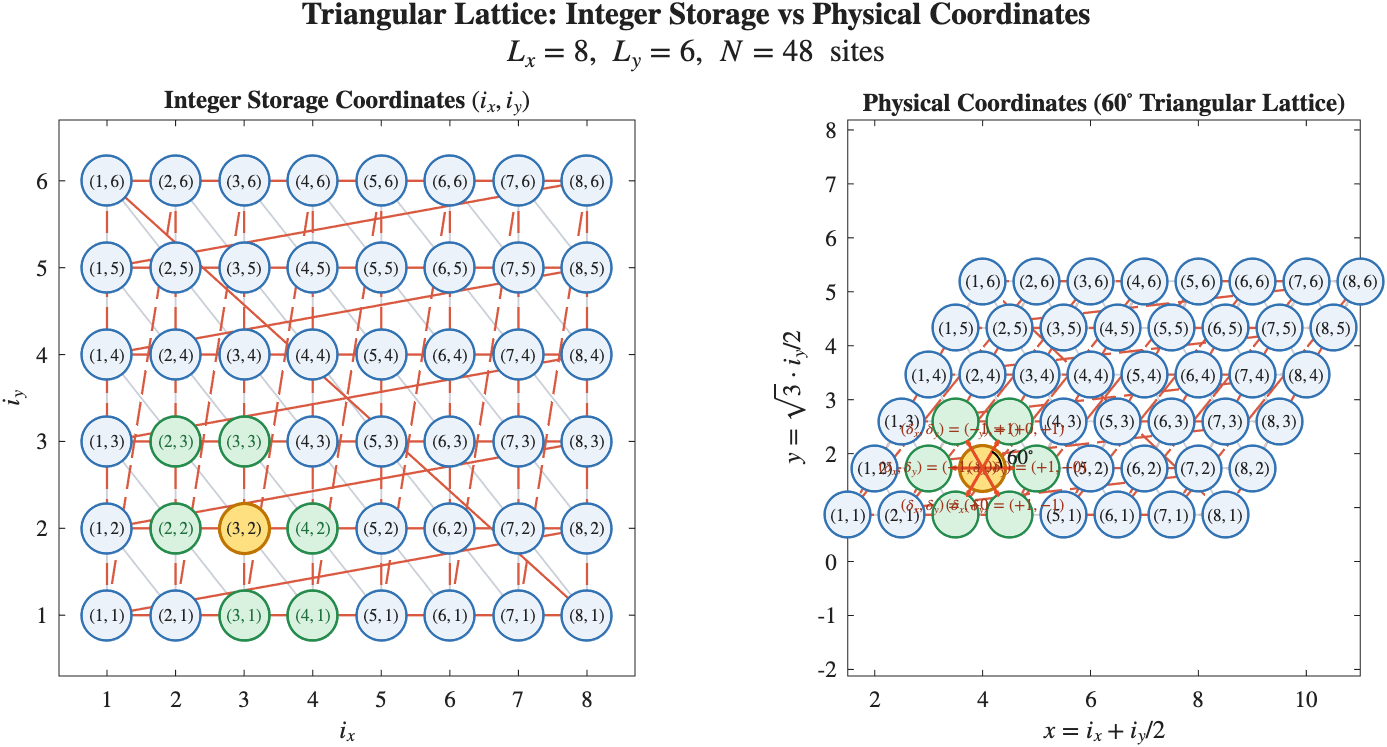
\includegraphics[width=\textwidth]{PBC.png}
\caption{Schematic of the $8 \times 6$ triangular lattice with periodic
boundary conditions. Each site has six nearest neighbours, and the
stripe-phase ground state is shown in blue and white.}
\end{figure}

\subsubsection{Stripe-Phase Initialisation}

\begin{equation}
    \sigma_i^{(0)} = \begin{cases}
        1 & \text{if } i_y \text{ is odd},\\
        0 & \text{if } i_y \text{ is even}.
    \end{cases}
    \label{eq:stripe_init}
\end{equation}

This requires $L_y$ to be even (satisfied by $L_y = 6$) to ensure
$\Nocc = N/2$ exactly.


\subsubsection{Running-Sum Time Average}

Rather than storing the full trajectory $\{\COHt{t}\}$,
the time average is accumulated incrementally:
\begin{equation}
    S \;\leftarrow\; S + \COH(\sigma^{(t)}), \qquad
    \avgE{\COH}(T) = S / N_{\mathrm{sample}}.
    \label{eq:running_sum}
\end{equation}
This requires $O(1)$ additional memory and is numerically stable.

\subsubsection{Low-Temperature Effective Non-Mixing and Sequential Annealing}

At very low temperatures, the Metropolis acceptance rate for
energy-raising moves satisfies
\begin{equation}
    e^{-\beta\Delta E} \leq e^{-\beta\varepsilon}
    = e^{-83.4} \approx 10^{-36}
    \quad \text{at } T = 10\,\mathrm{K},
\end{equation}
where $\Delta E = n\varepsilon$ ($n \geq 1$) is a small integer
multiple of $\varepsilon$.

We emphasise an important distinction.
The chain remains theoretically irreducible and aperiodic at all
temperatures (as established in Section~2), so ergodicity in the
strict mathematical sense is never broken.
What occurs at low temperature is \emph{effective non-mixing}: the
mixing time between metastable basins grows exponentially in
$\beta\varepsilon$, so that a chain initialised from a random
configuration ($C_{\mathrm{OH}}^B \approx 3$) becomes trapped in
an incorrect basin on any feasible simulation timescale.

\begin{definition}[Practical Ergodicity Breaking]
A Markov chain is said to exhibit \emph{practical ergodicity breaking}
at temperature $T$ if the inter-basin mixing time $\tau_{\mathrm{mix}}(T)$
exceeds the available simulation time, preventing convergence to
$\pi_{\mathrm{eq}}$ in practice.
\end{definition}

\textbf{Solution -- Sequential Annealing.}
The chain is initialised from the stripe-phase ground state
($C_{\mathrm{OH}}^B = 2$) outside the temperature loop, and
temperatures are scanned from high to low, passing the current
configuration directly to the next temperature.

The mechanism is the following.
At high temperatures, $\beta\varepsilon \ll 1$ and the chain mixes
efficiently across configuration space, so the ergodic theorem
applies within feasible simulation time.
As the temperature decreases, the system is guided continuously
into the correct low-energy basin.
At each subsequent temperature step the configuration is already
close to $\pi_{\mathrm{eq}}$, so only a short equilibration suffices.

The true role of sequential annealing is therefore not to
``restore ergodicity'' (which is never lost in the mathematical
sense), but to \emph{exploit the effective ergodicity at high
temperature} to pre-position the chain in the correct basin,
avoiding the exponentially slow inter-basin exploration that
would be required if the chain were initialised randomly at
low temperature.

\subsection{Computational Parameters}

\begin{table}[H]
\centering
\caption{Simulation parameters used in the production run.}
\label{tab:params}
\begin{tabular}{llr}
\toprule
Parameter & Symbol & Value \\
\midrule
Lattice size & $L_x \times L_y$ & $6 \times 4$ \\
Total sites & $N$ & 24 \\
Proton count & $\Nocc$ & 12 \\
NN repulsion energy & $\Eeps$ & 71.869\,meV \\
Boltzmann constant & $\kB$ & 0.08617\,meV\,K$^{-1}$ \\
Temperature range & $T$ & 10--300\,K \\
Number of $T$ points & $n_T$ & 1\,000 \\
Burn-in steps & $N_{\mathrm{equil}}$ & 5\,000 \\
Production steps & $N_{\mathrm{sample}}$ & 1\,000\,000 \\
\bottomrule
\end{tabular}
\end{table}

%================================================================
\section{Results}
\label{sec:results}
\begin{figure}[H]
\centering
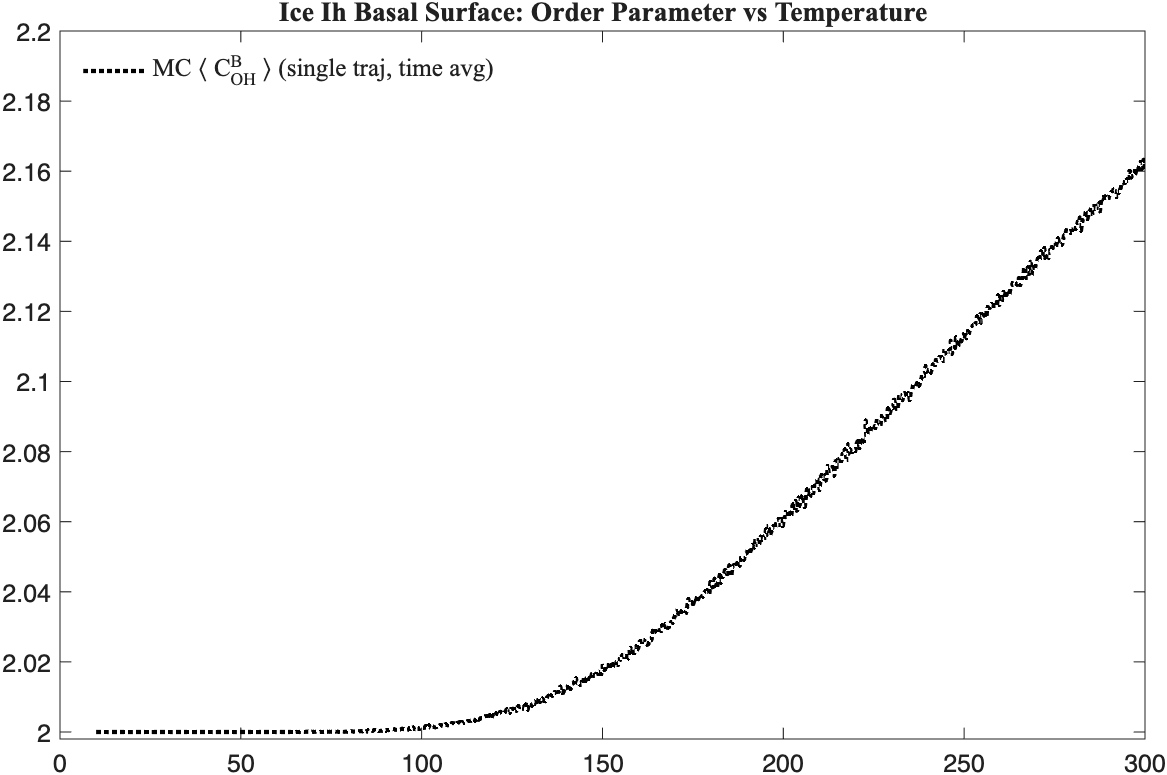
\includegraphics[width=0.8\textwidth]{original fig24.png}
\caption{Monte Carlo results for $\avgE{\COH}$ vs $T$. The error bars are estimated from the integrated autocorrelation time.}
\end{figure}

\hfill

Because of the MC random error, the curve is not perfectly smooth. In order to cancel out the noise and reveal the underlying trend, we apply a fitting procedure to the data. We choose 10-th order polynomial function. The fitted curve is shown in the following figure.

\begin{figure}[H]
\centering
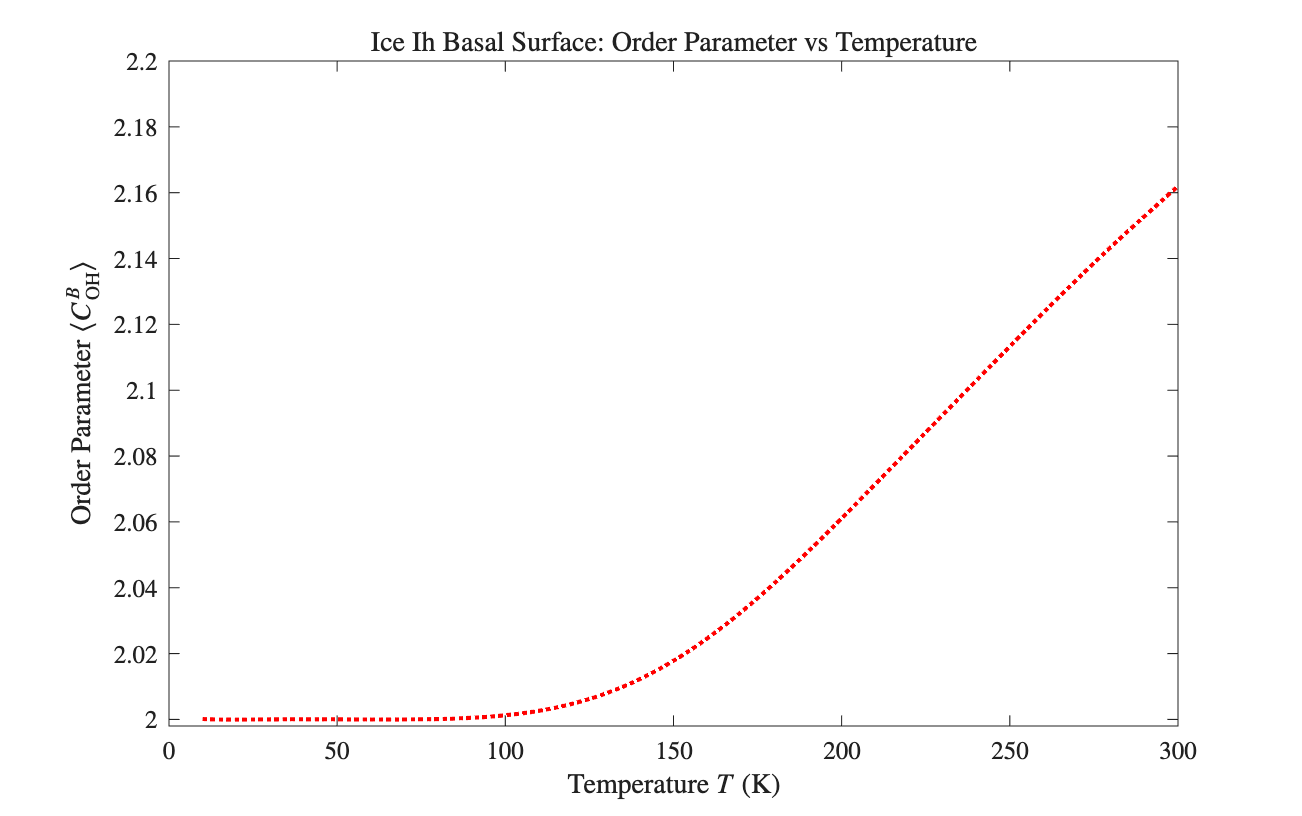
\includegraphics[width=0.8\textwidth]{fit24.png}
\caption{Fitted curve for $\avgE{\COH}$ vs $T$ using
a 10-th order polynomial.}
\end{figure}

%================================================================
% Bibliography
%================================================================
% \bibliographystyle{unsrtnat}  % not needed without natbib

% \begin{thebibliography}{99}

% \bibitem{pan2010}
% D.~Pan, L.-M.~Liu, G.~A.~Tribello, B.~Slater, A.~Michaelides, E.~Wang,
% \textit{Surface energy and surface proton order of the ice Ih basal and prism surfaces},
% J.~Phys.:~Condens.~Matter \textbf{22}, 074209 (2010).

% \bibitem{wannier1950}
% G.~H.~Wannier,
% \textit{Antiferromagnetism. The triangular Ising net},
% Phys.~Rev.\ \textbf{79}, 357 (1950).

% \bibitem{fletcher1992}
% N.~H.~Fletcher,
% \textit{Reconstruction of ice surfaces},
% Phil.~Mag.~B \textbf{66}, 109 (1992).

% \bibitem{kawasaki1966}
% K.~Kawasaki,
% \textit{Diffusion constants near the critical point for time-dependent
% Ising models},
% Phys.~Rev.\ \textbf{145}, 224 (1966).

% \bibitem{metropolis1953}
% N.~Metropolis, A.~W.~Rosenbluth, M.~N.~Rosenbluth, A.~H.~Teller, E.~Teller,
% \textit{Equation of state calculations by fast computing machines},
% J.~Chem.~Phys.\ \textbf{21}, 1087 (1953).

% \bibitem{flyvbjerg1989}
% H.~Flyvbjerg, H.~G.~Petersen,
% \textit{Error estimates on averages of correlated data},
% J.~Chem.~Phys.\ \textbf{91}, 461 (1989).

% \bibitem{levin2009}
% D.~A.~Levin, Y.~Peres, E.~L.~Wilmer,
% \textit{Markov Chains and Mixing Times},
% American Mathematical Society (2009).

% \bibitem{buch2008}
% V.~Buch, H.~Groenzin, I.~Li, M.~J.~Shultz, E.~Tosatti,
% \textit{Proton order in the ice crystal surface},
% Proc.~Natl Acad.~Sci.~USA \textbf{105}, 5969 (2008).

% \end{thebibliography}

%================================================================
% Appendices
%================================================================
\appendix

%----------------------------------------------------------------
% \section{Proof of the Ergodic Theorem for Finite Markov Chains}
% \label{app:ergodic}
% %----------------------------------------------------------------

% [TODO: Include a self-contained proof (or a precise reference) for the
% ergodic theorem \eqref{eq:ergodic_theorem} in the finite-state,
% irreducible, aperiodic case.
% Key steps:
% (1) Unique stationary distribution $\Peq$ exists by Perron--Frobenius.
% (2) Birkhoff's ergodic theorem for Markov chains gives almost-sure
%     convergence of the time average.
% (3) The $L^2$ convergence rate is $O(1/\sqrt{N_{\mathrm{sample}}})$
%     up to autocorrelation corrections.]

% %----------------------------------------------------------------
% \section{Integrated Autocorrelation Time}
% \label{app:autocorr}
% %----------------------------------------------------------------

% [TODO: Define the normalised autocorrelation function of $\COH$:
% \begin{equation}
%     \rho(s) \;=\;
%     \frac{\mathrm{Cov}\!\left(\COHt{t}, \COHt{t+s}\right)}
%          {\mathrm{Var}\!\left(\COHt{t}\right)},
%     \label{eq:acf}
% \end{equation}
% and the integrated autocorrelation time:
% \begin{equation}
%     \tau_{\mathrm{int}} \;=\; \frac{1}{2} + \sum_{s=1}^{\infty} \rho(s).
%     \label{eq:tauint}
% \end{equation}
% Explain how $\tau_{\mathrm{int}}$ relates to the effective sample size
% $N_{\mathrm{eff}} = N_{\mathrm{sample}} / (2\tau_{\mathrm{int}})$
% and to the Flyvbjerg--Petersen blocking estimator.]

% %----------------------------------------------------------------
% \section{MATLAB Source Code}
% \label{app:code}
% %----------------------------------------------------------------

% [TODO: Include your production MATLAB code here, or a key excerpt.
% Use the \texttt{lstlisting} environment:]

% \begin{lstlisting}[caption={Core MC loop (excerpt from \texttt{COH\_vs\_T\_single.m})},
%                    label={lst:core}]
% for iT = 1:n_T
%     T    = T_list(iT);
%     beta = 1.0 / (kB_meV_per_K * T);

%     % Equilibration: config inherited from previous T
%     for step = 1:N_equil
%         [occ, occ_idx, free_idx] = mc_swap( ...
%             occ, occ_idx, free_idx, nn_list, N_occ, beta, epsilon_meV);
%     end

%     % Time average  ==  ensemble average  (ergodic theorem)
%     COH_sum = 0.0;
%     for step = 1:N_sample
%         [occ, occ_idx, free_idx] = mc_swap( ...
%             occ, occ_idx, free_idx, nn_list, N_occ, beta, epsilon_meV);
%         occ_rows = nn_list(occ, :);
%         COH_sum  = COH_sum + double(sum(occ(occ_rows(:)))) / N_occ;
%     end
%     COH_mean(iT) = COH_sum / N_sample;
% end
% \end{lstlisting}

\section{Working with AI Assistant}
\label{app:ai}

\hfill

The background about the application of MC algorithm in this project was understood by discussing with ChatGPT-5.5 and Gemini 3.1 Pro.

The fundamental theoretical formula derivations and proofs were checked by ChatGPT-5.5 and Claude Sonnet4.6.

The optimization of algorithms like Low-Temperature Sequential Annealing were built with ChatGPT-5.5 and Claude Sonnet4.6.

The code was generated and debugged by the assistance of Claude Sonnet4.6 with the prompts about the fundamental theoretical formulas and the flow of the program.

The framework of the report was generated by Claude Sonnet4.6, and the typo-checking was done by them.

\end{document}